%!LW recipe=latexmk-xelatex
\documentclass[compress]{beamer}

\usetheme[block=fill]{metropolis}

\usepackage{graphicx} % Allows including images
\usepackage{amsmath,amsfonts,amsthm,amssymb}
\usepackage{color}
\usepackage{xcolor,cancel}
\usepackage{tcolorbox}
\setbeamercolor{colorBoxStuff}{fg=black, bg=gray!30!white}
%\setitemize{label=\usebeamerfont*{itemize item}%
%	\usebeamercolor[fg]{itemize item}
%	\usebeamertemplate{itemize item}}
\definecolor{mDarkBrown}{HTML}{604c38}
\definecolor{mDarkTeal}{HTML}{23373b}
\definecolor{mLightBrown}{HTML}{EB811B}
\definecolor{mMediumBrown}{HTML}{C87A2F}
\definecolor{mygreen}{HTML}{98C2B9}
\definecolor{myyellow}{HTML}{DFD79C}
\definecolor{myblue}{HTML}{8CA7CC}
\definecolor{kern}{HTML}{8CC2B7}


\usepackage{float}
\usepackage{framed}
\usepackage{epsfig}
\usepackage{graphicx}
\usepackage{subcaption}
\usepackage{ulem}
\usepackage{hhline}
\usepackage{multirow}
\usepackage{comment}   
\usepackage{bbm}
\usepackage{tikz}   
\def\Put(#1,#2)#3{\leavevmode\makebox(0,0){\put(#1,#2){#3}}}
\newcommand*\mystrut[1]{\vrule width0pt height0pt depth#1\relax}
\newcommand{\eqdef}{\mathbin{\stackrel{\rm def}{=}}}
\usepackage{hyperref}


\newcommand{\bs}[1]{\boldsymbol{#1}}
\newcommand{\bv}[1]{\mathbf{#1}}
\newcommand{\R}{\mathbb{R}}
\newcommand{\E}{\mathbb{E}}

\DeclareMathOperator*{\argmin}{arg\,min}
\DeclareMathOperator*{\argmax}{arg\,max}
\DeclareMathOperator{\nnz}{nnz}
\DeclareMathOperator{\vol}{vol}
\DeclareMathOperator{\diag}{diag}
\DeclareMathOperator{\Var}{Var}
\DeclareMathOperator{\sinc}{sinc}
\DeclareMathOperator{\sign}{sign}
\DeclareMathOperator{\dist}{dist}
\DeclareMathOperator{\mv}{mv}
\DeclareMathOperator{\sgn}{sgn}
\DeclareMathOperator{\step}{step}
\DeclareMathOperator{\gap}{gap}
\DeclareMathOperator{\poly}{poly}
\DeclareMathOperator{\tr}{tr}
\DeclareMathOperator{\orth}{orth}
\newcommand{\norm}[1]{\|#1\|}
\captionsetup[subfigure]{labelformat=empty}
\captionsetup[figure]{labelformat=empty}
\DeclareMathOperator*{\lmin}{\lambda_{min}}
\DeclareMathOperator*{\lmax}{\lambda_{max}}

\newcommand{\specialcell}[2][c]{%
  \begin{tabular}[#1]{@{}c@{}}#2\end{tabular}}
\newcommand{\specialcellleft}[2][c]{%
\begin{tabular}[#1]{@{}l@{}}#2\end{tabular}
}

\newtheorem{claim}[theorem]{Claim}
%\newtheorem{corollary}[theorem]{Corollary}

\usepackage{tabstackengine}
\stackMath


%----------------------------------------------------------------------------------------
%	TITLE PAGE
%----------------------------------------------------------------------------------------

\title{CS-GY 6763: Lecture 4 \\  High Dimensional Geometry, the Johnson-Lindenstrauss Lemma}
\author{NYU Tandon School of Engineering, Prof. Christopher Musco}
\date{}

\begin{document}

\begin{frame}
	\titlepage 
\end{frame}

\metroset{titleformat=smallcaps}

\begin{frame}
	\frametitle{unifying theme of the course}
	\begin{center}
		\textbf{How do we deal with data (vectors) in high-dimensions?}
	\end{center}
\begin{itemize}
	\item High-dimensional similarity search.  
	\item Iterative methods for optimizing functions in high-dimensions.
	\item SVD + low-rank approximation to find and visualize low-dimensional structure.
	\item Convert large graphs to high-dimensional vector data to uncover interesting things. 
\end{itemize}
\end{frame}

\begin{frame}
	\frametitle{high dimensional is not like low dimensional}
	\begin{center}
		\textbf{Often visualize data and algorithms in 1,2, or 3 dimensions.}
		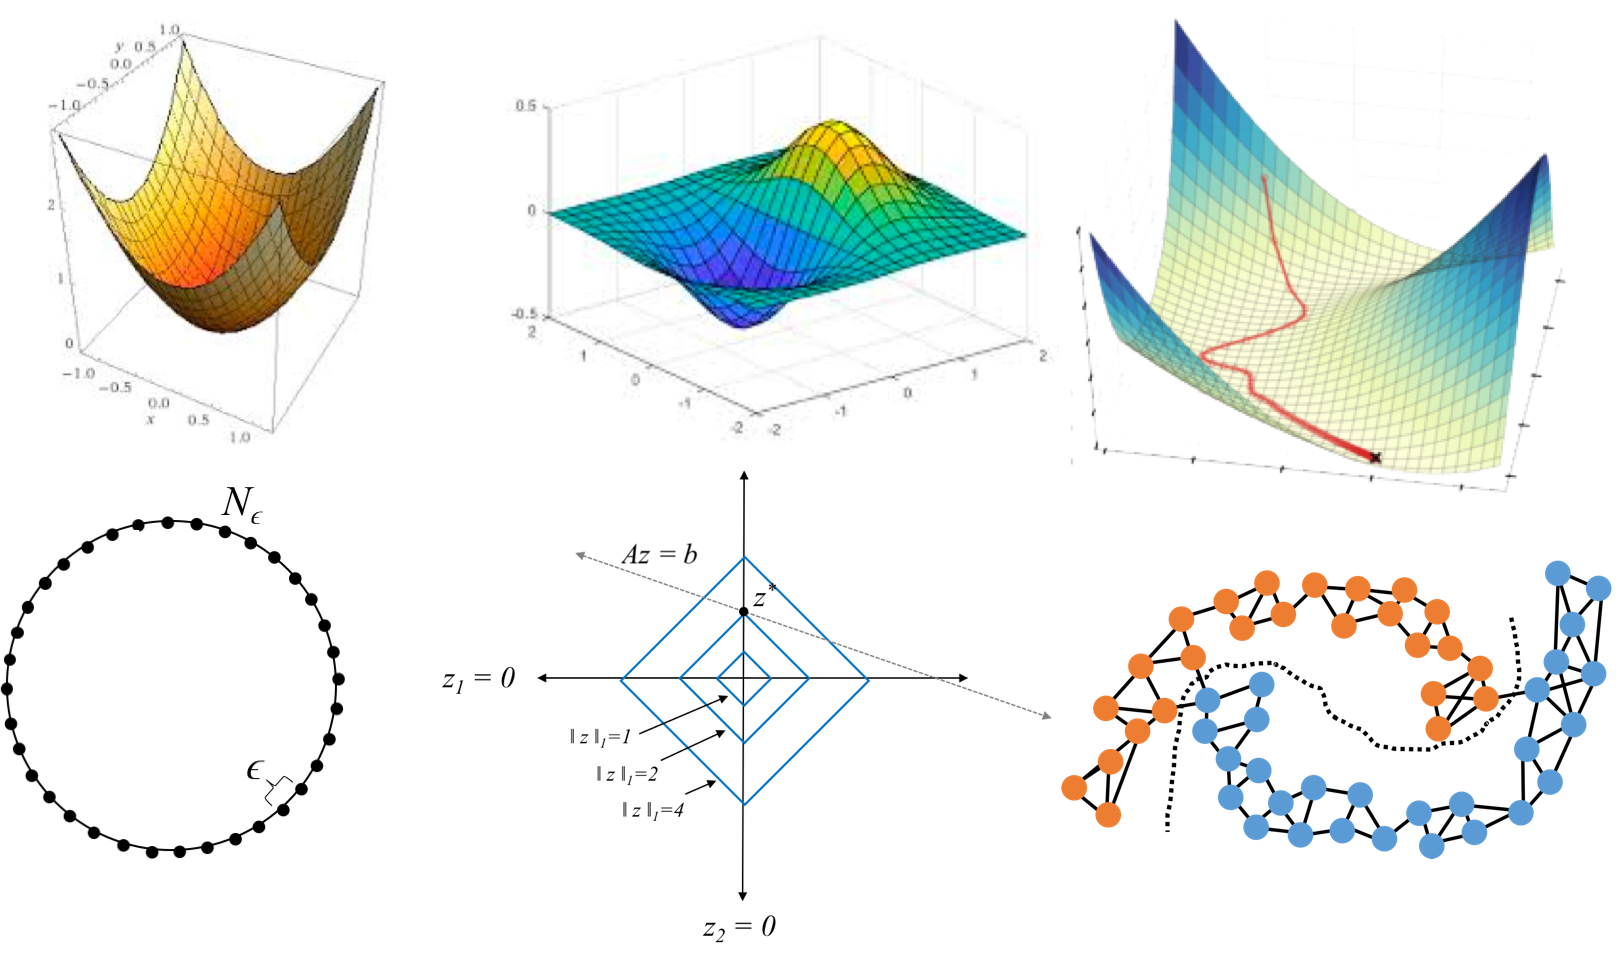
\includegraphics[width=.8\textwidth]{lowdim_visualizations.png}
		
		\textbf{First part of lecture:} Prove that high-dimensional space looks \textbf{\alert{very different}} from low-dimensional space. These images are rarely very informative! 
	\end{center}
\end{frame}

\begin{frame}
	\frametitle{sketching and dimensionality reduction}
	\begin{center}
		\textbf{Second part of lecture:} Ignore our own advice. 
	\end{center}
		Learn about \alert{\textbf{sketching, aka dimensionality reduction}} techniques that seek to approximate high-dimensional vectors with much lower dimensional vectors. 
		\begin{itemize}
			\item Johnson-Lindenstrauss lemma for $\ell_2$ space.
			\item MinHash for binary vectors (next class) . 
		\end{itemize}
		\begin{center}
			\vspace{-.75em}
		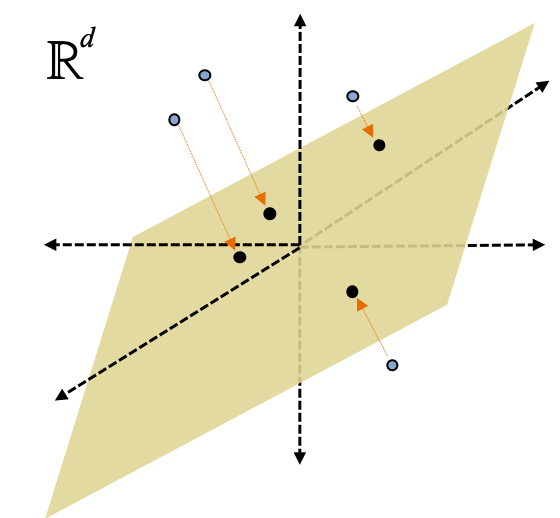
\includegraphics[width=.3\textwidth]{random_projection.png}
		\vspace{-.75em}
		\end{center}
		
		First part of lecture should help you understand the potential and limitations of these methods. 
\end{frame}

\begin{frame}[t]
	\frametitle{orthogonal vectors}
		\textbf{Recall the inner product between two $d$ dimensional vectors:}
		\begin{align*}
			\langle \bv{x},\bv{y} \rangle = \bv{x}^T\bv{y} = \bv{y}^T\bv{x} = \sum_{j=1}^d x[j]y[j]
		\end{align*}
	\begin{center}
		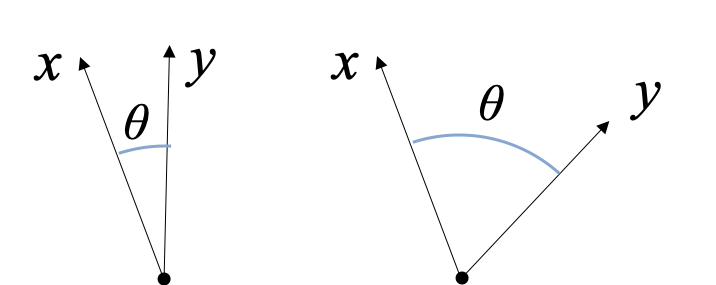
\includegraphics[width=.7\textwidth]{inner_product.png}
	\end{center}
	
	\begin{align*}
		\langle \bv{x},\bv{y} \rangle = \cos(\theta)\cdot\|\bv{x}\|_2\cdot\|\bv{y}\|_2
	\end{align*}
\end{frame}

\begin{frame}[t]
	\frametitle{orthogonal vectors}
	\begin{center}
		\alert{What is the largest set of \textbf{mutually orthogonal} unit vectors $\bv{x}_1, \ldots, \bv{x}_t$ in $d$-dimensional space? I.e. with inner product $|\bv{x}_i^T\bv{x}_j| = 0$ for all $i$, $j$.}
		\begin{center}
			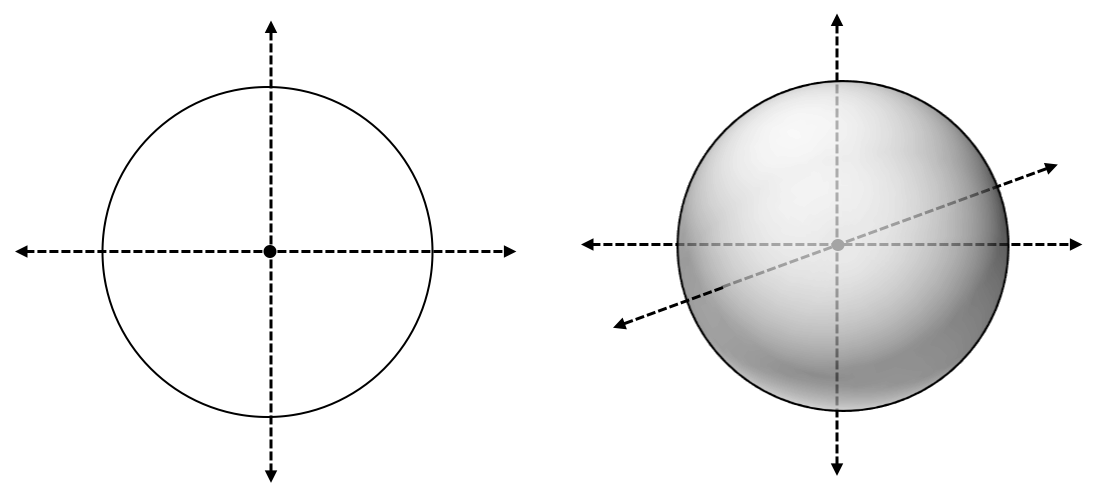
\includegraphics[width=.8\textwidth]{dimension_vis.png}
		\end{center}
	\end{center}
	
	
\end{frame}

\begin{frame}[t]
	\frametitle{orthogonal vectors}
	\begin{center}
		\alert{What is the largest set \textbf{nearly orthogonal} unit vectors $\bv{x}_1, \ldots, \bv{x}_t$ in $d$ dimensions. I.e., with inner product $|\bv{x}_i^T\bv{x}_j| \leq \epsilon$ for all $i$, $j$. Consider the case when $\epsilon$ is a constant. E.g. $\epsilon = 1/10$. }

			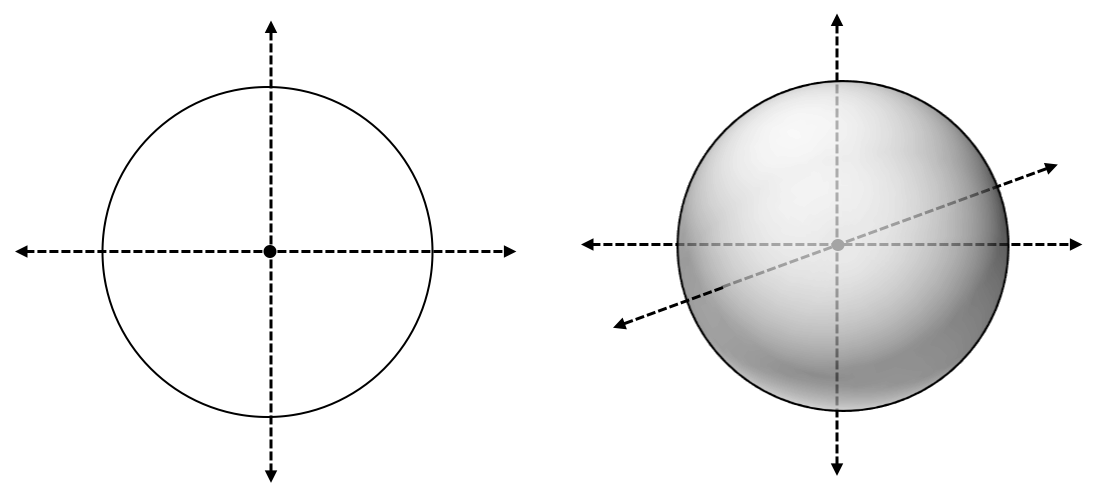
\includegraphics[width=.8\textwidth]{dimension_vis.png}
	\end{center}
		

\end{frame}

\begin{frame}[t]
	\frametitle{orthogonal vectors}
	\begin{center}
			\alert{What is the largest set \textbf{nearly orthogonal} unit vectors $\bv{x}_1, \ldots, \bv{x}_t$ in $d$ dimensions. I.e., with inner product $|\bv{x}_i^T\bv{x}_j| \leq \epsilon$ for all $i$, $j$. Consider the case when $\epsilon$ is a constant. E.g. $\epsilon = 1/10$. }
		\vspace{10em}
		
		1. $d$ \hspace{3em}2. $\Theta(d)$ \hspace{3em}3. $\Theta(d^2)$ \hspace{3em}4. $2^{\Theta(d)}$   
	\end{center}
\end{frame}

\begin{frame}[t]
	\frametitle{orthogonal vectors}
		\textbf{Claim:} There is an exponential number of nearly orthogonal unit vectors in $d$ dimensional space  (i.e., $\sim 2^d$).

		\textbf{Formally:} In $d$-dimensional space, there are $2^{\Theta(\epsilon^2 d)}$ unit vectors with all pairwise inner products $\leq \epsilon$. 
		
		\textbf{Proof strategy:} Use the \alert{Probabilistic Method}! For $t =  2^{\Theta(\epsilon^2 d)}$, define a random process which generates random vectors $\bv{x}_1, \ldots, \bv{x}_t$ that are unlikely to have large inner product.
		\begin{enumerate}
			\item Claim that, with non-zero probability, $|\bv{x}_i^T\bv{x}_j| \leq \epsilon$ for all $i$, $j$.
			
			\item Conclude that there must exists \emph{some} set of $t$ unit vectors with all pairwise inner-products  bounded by $\epsilon$. 
		\end{enumerate}
\end{frame}


\begin{frame}[t]
	\frametitle{probabilistic method}
	\textbf{Claim:} There is an exponential number (i.e., $ 2^{\Theta(d)}$) of nearly orthogonal unit vectors in $d$ dimensional space.
	
	\textbf{Proof:} Let $\bv{x}_1, \ldots, \bv{x}_t$ all have independent random entries, each set to $\pm \frac{1}{\sqrt{d}}$ with equal probability. 
	\begin{itemize}
		\item $\|\bv{x}_i\|_2^2 = $
		\vspace{2em}
		\item $\E[\bv{x}_i^T\bv{x}_j]=$
		\vspace{2em}
		\item $\Var[\bv{x}_i^T\bv{x}_j]=$
	\end{itemize}
\end{frame}

\begin{frame}[t]
	\frametitle{informal proof}
	Let $Z = \bv{x}_i^T\bv{x}_j = \sum_{i=1}^d C_i$ where each $C_i$ is random $\pm \frac{1}{d}$.
	
	
	$Z$ is a sum of many i.i.d. random variables, so looks approximately Gaussian. Roughly, we expect that:
	\begin{align*}
		\Pr[|Z - \E Z| \geq \alpha\cdot \sigma] \leq O(e^{-\alpha^2})
	\end{align*}
\vspace{8em}

By a union bound, we can claim that the above holds for all pairs in a set of size:
\end{frame}

\begin{frame}
	\frametitle{formal proof}
	Use an exponential concentration inequality!
	\begin{theorem}[Chernoff Bound]
		Let $X_1,X_2,\ldots,X_d$ be independent $\{0,1\}$-valued random variables and let
		$S = \sum_{i=1}^{d} X_i$. We have for any $\epsilon < 1$ :
		\begin{align*}
			\Pr[|S - \E[S]| \geq \epsilon\E[S]] \leq 2e^{\frac{-\epsilon^2\E[S]}{3}}.
		\end{align*}
	\end{theorem} 
Does not immediately apply because we have random variables that are $\pm 1/{d}$, not $0,1$.

	\textbf{Common trick: shift and scale to transform to the binary case}.
\end{frame}

\begin{frame}[t]
	\frametitle{formal proof}

	\begin{align*}
		\bv{x}_i^T\bv{x}_j = Z = \sum_{i=1}^d C_i &= \frac{2}{d} \sum_{i=1}^d \frac{d}{2}\cdot C_i\\
		&= \frac{2}{d}\cdot \left(\sum_{i=1}^d B_i - 1/2\right)\\
		&= \frac{2}{d}\cdot \left(-\frac{d}{2} + \sum_{i=1}^d B_i \right)
	\end{align*}
	where each $B_i$ is uniform in $\{0,1\}$. 
\end{frame}



\begin{frame}[t]
		\frametitle{formal proof}
	\begin{align*}
		\bv{x}_i^T\bv{x}_j = Z = \frac{2}{d}\cdot \left(-\frac{d}{2} + \sum_{i=1}^d B_i \right)
	\end{align*}
	where each $B_i$ is uniform in $\{0,1\}$. 
	
	\begin{align*}
		\Pr[|Z| > \epsilon] &= \Pr\left[\sum_{i=1}^d B_i \geq \frac{d}{2} + \frac{\epsilon d}{2}\right] +\Pr\left[\sum_{i=1}^d B_i \leq \frac{d}{2} - \frac{\epsilon d}{2}\right ]\\
		& = \Pr\left[\sum_{i=1}^d B_i \geq (1+\epsilon)\E\left[\sum_{i=1}^d B_i\right ]\right] \\ &\hspace{3em}+ \Pr\left[\sum_{i=1}^d B_i \leq (1-\epsilon)\E\left[\sum_{i=1}^d B_i\right ]\right]
	\end{align*}
\end{frame}

\begin{frame}
	\frametitle{chernoff bound}
	\begin{theorem}[Chernoff Bound]
		Let $X_1,X_2,\ldots,X_d$ be independent $\{0,1\}$-valued random variables and let
		$S = \sum_{i=1}^{d} X_i$. We have for any $\epsilon < 1$ :
		\begin{align*}
			\Pr[|S - \E[S]| \geq \epsilon\E[S]] \leq 2e^{\frac{-\epsilon^2\E[S]}{3}}.
		\end{align*}
	\end{theorem} 
	Apply with $X_1, \ldots, X_d = B_1, \ldots, B_d$:
	\begin{align*}
	\Pr[|S - \E[S]| \geq \epsilon\E[S]] \leq \hspace{5em}
\end{align*}
\end{frame}

\begin{frame}[t]
	\frametitle{probabilistic method}
	\textbf{Conclusion from Chernoff bound:}
	\begin{align*}
		\text{For \emph{any} $i,j$ pair, }\Pr[|\bv{x}_i^T\bv{x}_j| < \epsilon] \geq 1 -  2e^{-\epsilon^2 d/6}.
	\end{align*}
	By a union bound:
	\begin{align*}
	\text{For \emph{all} $i,j$ pairs simultaneously, }\Pr[|\bv{x}_i^T\bv{x}_j| < \epsilon] \geq 1- {t\choose 2} \cdot 2e^{-\epsilon^2 d/6} .
	\end{align*}
\end{frame}

\begin{frame}[t]
	\frametitle{orthogonal vectors}
	\textbf{Final result:} In $d$-dimensional space, there are $2^{\Theta(\epsilon^2 d)}$ unit vectors with all pairwise inner products $\leq \epsilon$. 
	
	\vspace{1em}
	\textbf{Corollary of proof:} \emph{Random vectors} tend to be far apart (and roughly equidistant) in high-dimensions.
	\vspace{3em}
	\begin{center}
		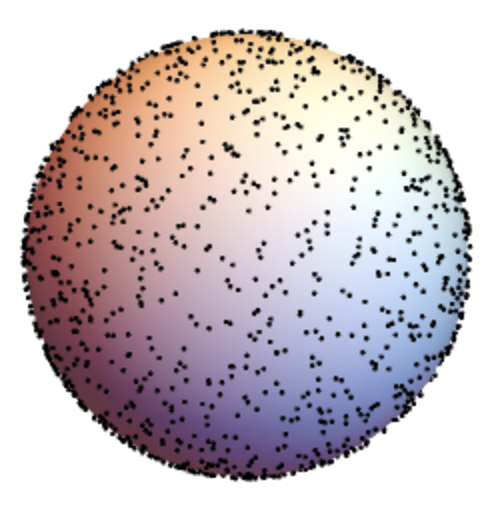
\includegraphics[width=.3\textwidth]{points_on_sphere.png}
	\end{center}
	
\end{frame}

\begin{frame}[t]
	\frametitle{curse of dimensionality}
	\alert{\textbf{Curse of dimensionality}}: Suppose we want to use e.g. $k$-nearest neighbors to learn a function or classify points in $\R^d$. If our data distribution is truly random, we typically need an exponential amount of data. 
	\begin{center}
		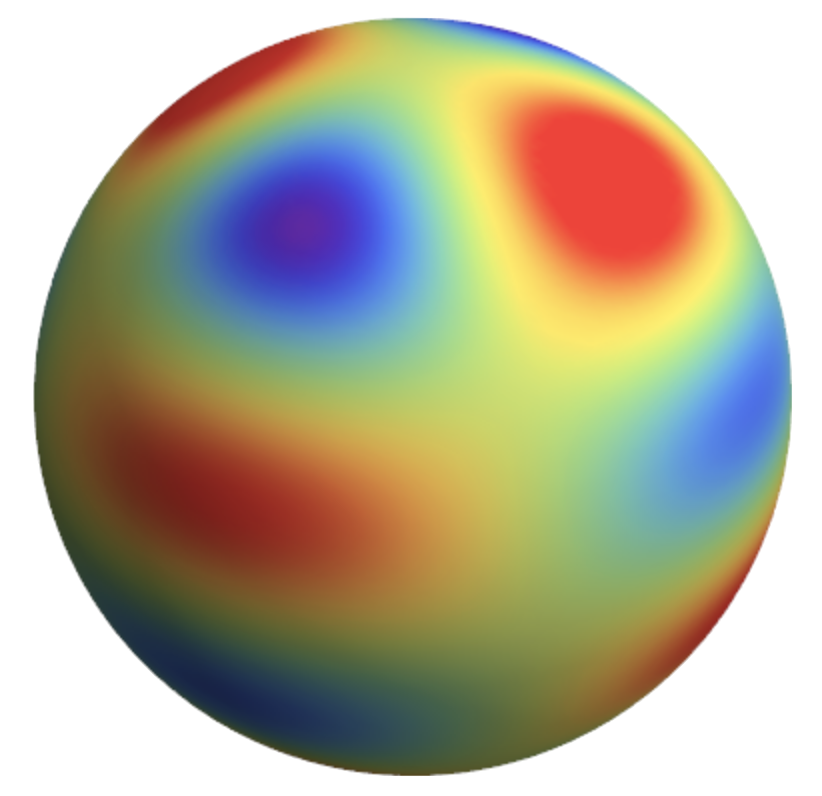
\includegraphics[width=.3\textwidth]{sphere_function.png}
	\end{center}
		\textbf{The existence of lower dimensional structure is our data is often the only reason we can hope to learn.}

\end{frame}

\begin{frame}[t]
	\frametitle{curse of dimensionality}
	\begin{center}
		\alert{\textbf{Low-dimensional structure}}. 
		\vspace{1em}
		
		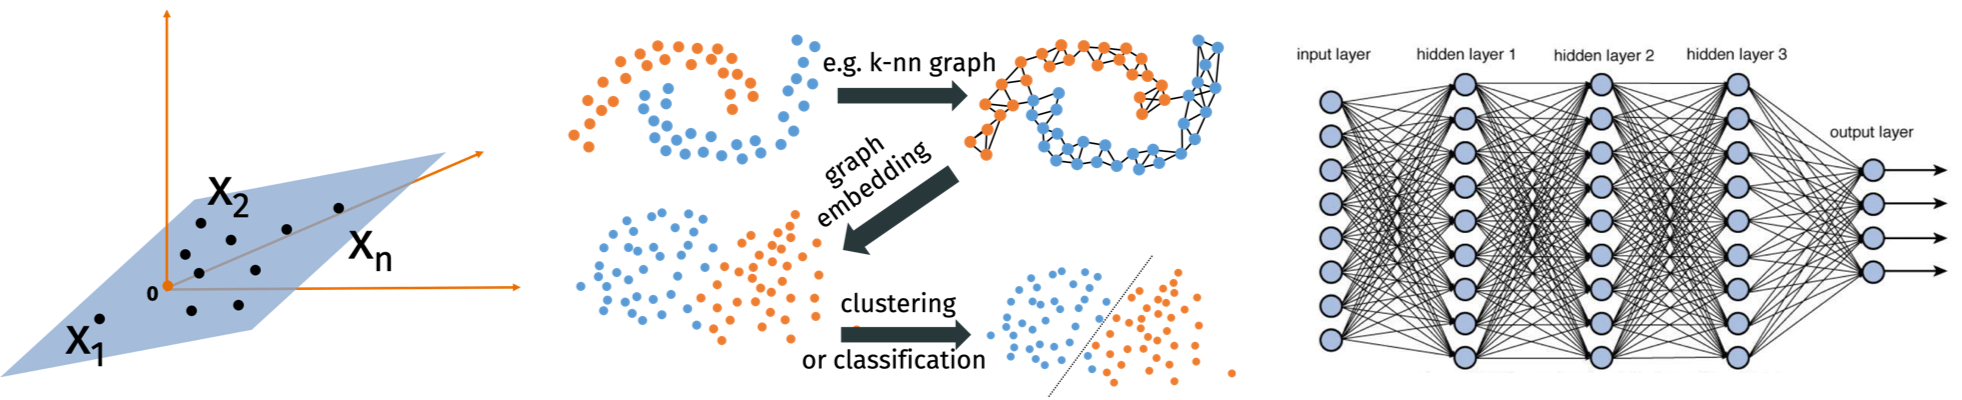
\includegraphics[width=\textwidth]{lowdim_structure.png}
		\vspace{1em}
		
		\textbf{For example, data lies on low-dimensional subspace, or does so after transformation. Or function can be represented by a restricted class of functions, like neural net with specific architecture.}
	\end{center}
\end{frame}

%\begin{frame}
%	\frametitle{value of many orthogonal vectors}
%	\begin{definition}[$(q,\epsilon)$-Restricted Isometry Property]
%		A matrix $\bv{A}$ satisfies $(q,\epsilon)$-RIP if, for all $\bv{x}$ with $\|\bv{x}\|_0 \leq q$, 
%		\begin{align*}
%		(1-\epsilon)\|\bv{x}\|_2^2 \leq \|\bv{A}\bv{x}\|_2^2 \leq  (1+\epsilon)\|\bv{x}\|_2^2.
%		\end{align*}
%	\end{definition}
%\begin{center}
%	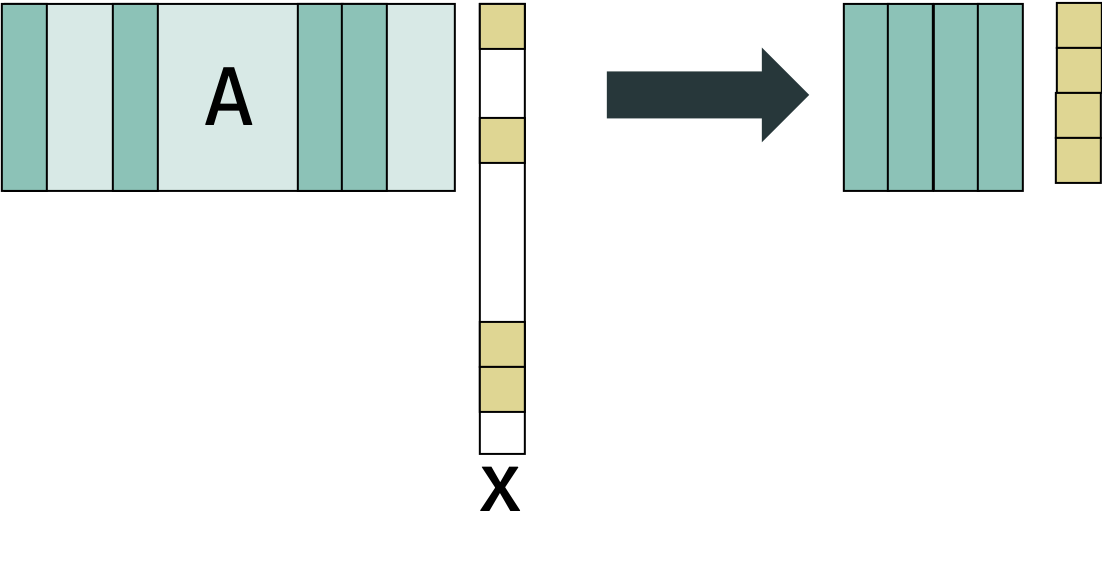
\includegraphics[width=.6\textwidth]{restricted_isom.png}
%	
%	Every subset of $k$ columns $\bv{U}\in \R^{m\times k}$ is approximate \emph{isometry}.
%	\begin{align*}
%		\bv{U}^T\bv{U} \approx \bv{I}.
%	\end{align*}
%\end{center}
%\end{frame}
%
%\begin{frame}
%	\frametitle{value of many orthogonal vectors}
%	If $\bv{U}^T\bv{U} \approx \bv{I}$, it better be that any two columns $\bv{u}_i, \bv{u}_j$ are approximately orthogonal.  
%	
%	\textbf{Deduce:} All pairs of columns in $\bv{A}$ are approximately orthogonal. 
%	
%	Think of $k$ as a constant: $k = O(1)$. We have $d$ nearly orthogonal vectors living in $O(k\log d) = \alert{O(\log d)}$ dimensional space.
%\end{frame}

\begin{frame}[t]
	\frametitle{unit ball in high dimensions}
	Let $\mathcal{B}_d$ be the unit ball in $d$ dimensions: \begin{align*}\mathcal{B}_d = \{\bv{x}\in \R^d: \|\bv{x}\|_2 \leq 1\}.\end{align*}
	\alert{What percentage of volume of $\mathcal{B}_d$ falls with $\epsilon$ of its surface?}
		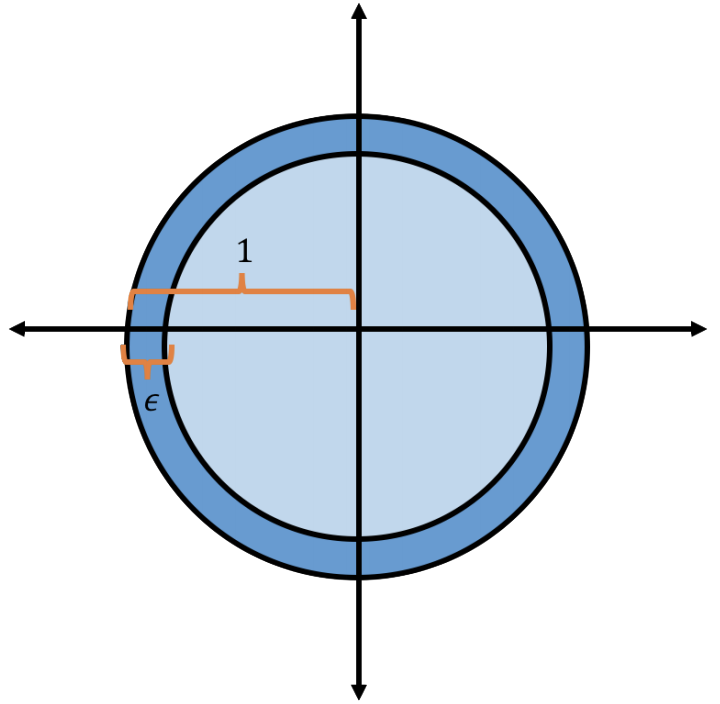
\includegraphics[width=.4\textwidth]{unitBall.png}
		
	Volume of radius $R$ ball is $\frac{\pi^{d/2}}{(d/2)!}\cdot R^d$. 
\end{frame}

\begin{frame}[t]
	\frametitle{isoperimetric inequality}
	All but a vanishing small $2^{-\Theta(\epsilon d)}$ fraction of a unit ball's volume is within $\epsilon$ of its surface.
	
	\textbf{Isoperimetric Inequality:} the ball has the minimum surface
	area/volume ratio of any shape.
	\begin{center}
	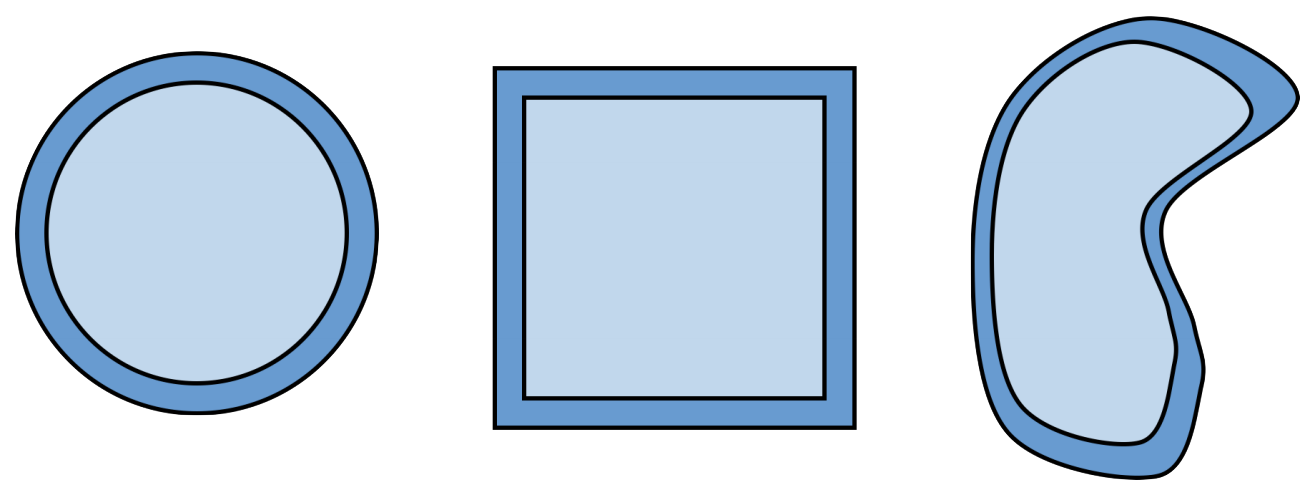
\includegraphics[width=.7\textwidth]{isoperimetry.png}
	\end{center}
	\begin{itemize}
	\item If we randomly sample points from any high-dimensional shape,
	nearly all will fall near its surface.
	\item  ‘All points are outliers.’ 
	\end{itemize}
\end{frame}

\begin{frame}[t]
	\frametitle{intuition}
	\begin{center}
		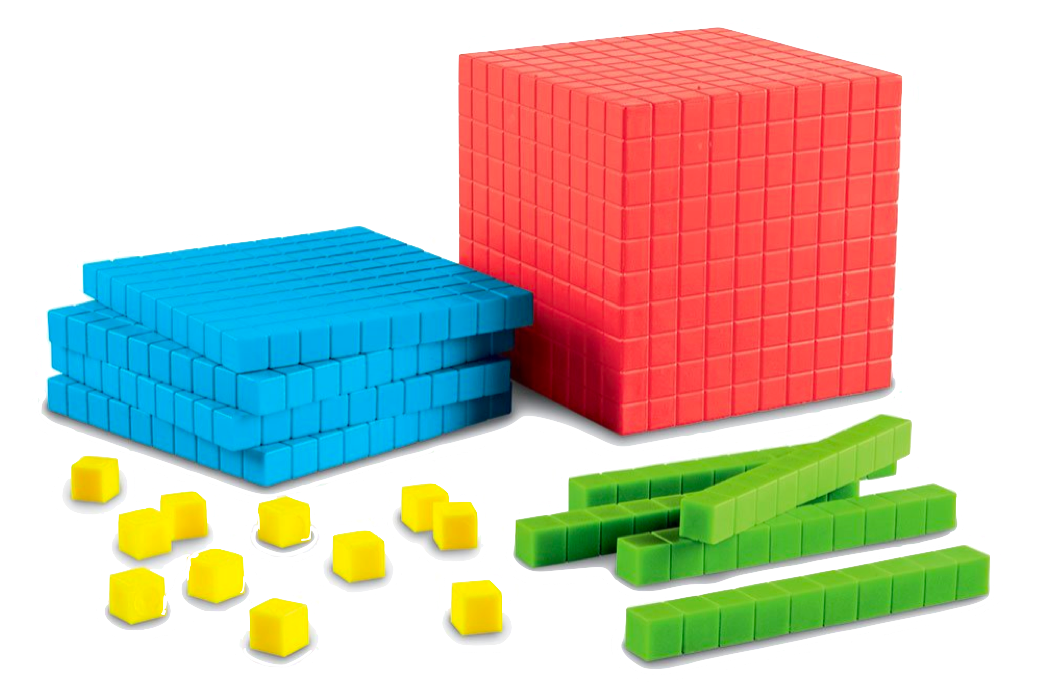
\includegraphics[width=.6\textwidth]{base10.png}
	\end{center}
	\vspace{-1em}
	1D: $\frac{\text{surface cubes}}{\text{total cubes}} = $
	\vspace{1em}

	2D: $\frac{\text{surface cubes}}{\text{total cubes}} = $
	\vspace{1em}
	
	3D: $\frac{\text{surface cubes}}{\text{total cubes}} = $
\end{frame}

\begin{frame}[t]
	\frametitle{slices of the unit ball}
	\alert{What percentage of the volume of $\mathcal{B}_d$ falls within $\epsilon$ of its equator?} 
	
	\begin{center}
		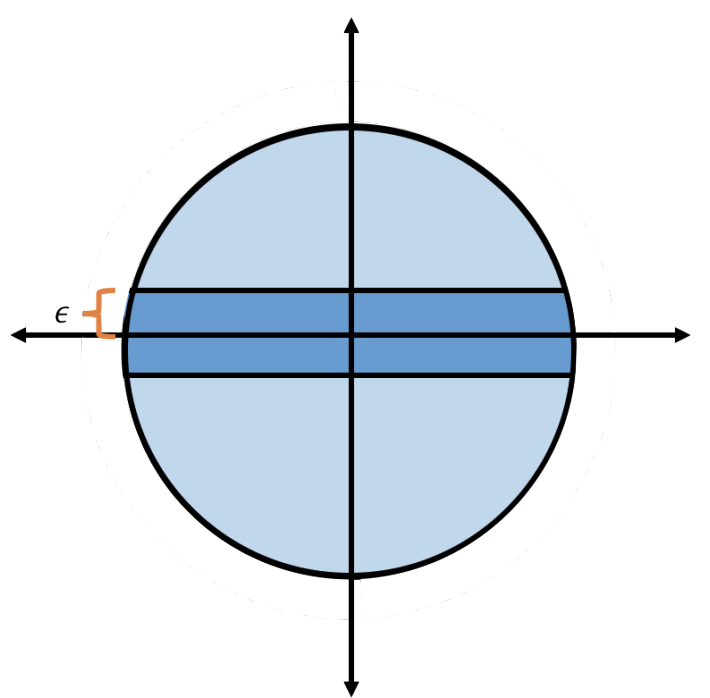
\includegraphics[width=.5\textwidth]{equator.png}
		
		$S = \{\bv{x}\in \mathcal{B}_d: |x_1|\leq \epsilon\}$
	\end{center}
\end{frame}

\begin{frame}[t]
	\frametitle{slices of the unit ball}
	\alert{What percentage of the volume of $\mathcal{B}_d$ falls within $\epsilon$ of its equator?} \textbf{Answer}: all but a $2^{-\Theta(\epsilon^2 d)}$ fraction.
	\vspace{-.5em}
	\begin{center}
		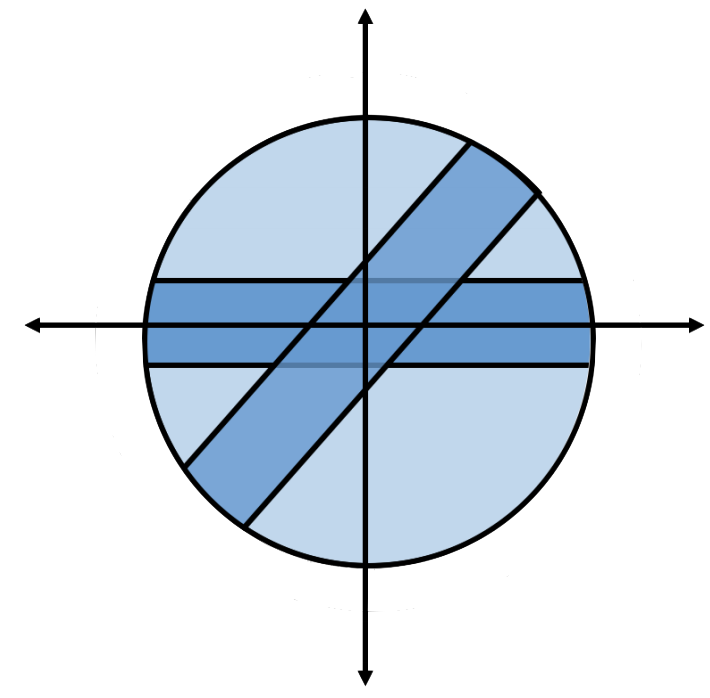
\includegraphics[width=.5\textwidth]{2equators.png}
		
		\vspace{-.5em}
		By symmetry, this is true for any equator: $S_{\bv{t}} = \{\bv{x}\in \mathcal{B}_d: \bv{x}^T\bv{t}\leq \epsilon\}$.
	\end{center}
\end{frame}

\begin{frame}[t]
	\frametitle{bizarre shape of unit ball}
	\begin{enumerate}
		\item $(1 -2^{-\Theta(\epsilon d)})$ fraction of volume lies $\epsilon$ close to surface. 
		\item $(1 -  2^{-\Theta(\epsilon^2 d)})$ fraction of volume lies $\epsilon$ close to any equator. 
	\end{enumerate}

	\begin{center}
	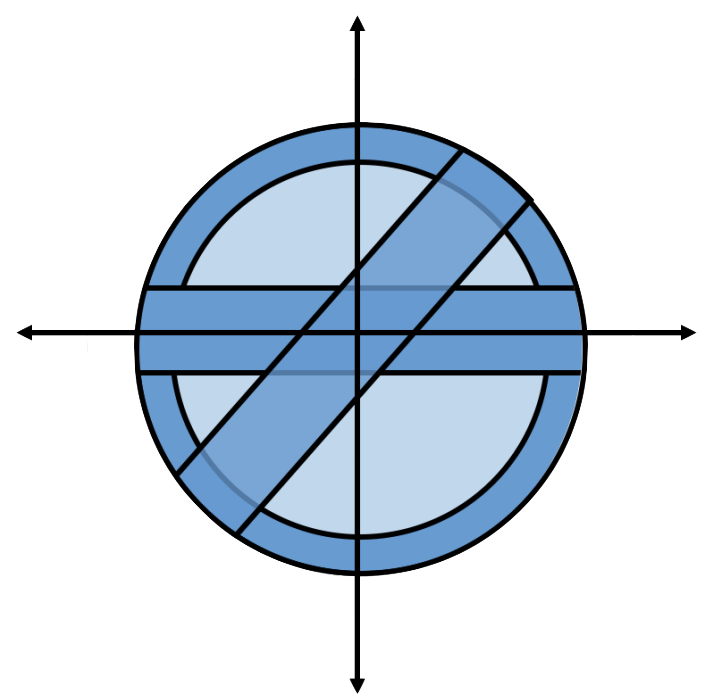
\includegraphics[width=.5\textwidth]{equators_surface.png}
	
	\textbf{\alert{High-dimensional ball looks nothing like 2D ball!}}
	\end{center}
\end{frame}

\begin{frame}[t]
	\frametitle{concentration at equator}
	\textbf{Claim:} All but a $2^{-\Theta(\epsilon^2 d)}$ fraction of the volume of the ball falls within $\epsilon$ of its equator. 
		
	\textbf{Equivalent:} If we draw a point $\bv{x}$ \emph{randomly} from the unit ball, $|x_1| \leq \epsilon$ with probability $\geq 1 - {2}^{-\Theta(\epsilon^2 d)}$. 
\end{frame}

\begin{frame}[t]
	\frametitle{concentration at equator}
	Let $\bv{w} = \frac{\bv{x}}{\|\bv{x}\|_2}$. Because $\|\bv{x}\|_2 \leq 1$,
\begin{align*}
\Pr\left[|x_1| \leq \epsilon\right] \geq \Pr\left[|w_1| \leq \epsilon\right].
\end{align*}
	\textbf{Claim:} $|w_1| \leq \epsilon$ with probability $\geq 1 - 2^{-\Theta(\epsilon^2 d)}$. This then proves our statement from the previous slide.
	\vspace{8em}

\alert{\textbf{How can we generate $\bv{w}$, which is a random vector taken from the unit \emph{sphere} (the surface of the ball)?}}
\end{frame}

\begin{frame}[t]
	\frametitle{important fact in high dimensional geometry}
	\textbf{Rotational Invariance of Gaussian distribution:}
	Let $\textbf{g}$ be a random Gaussian vector, with each entry drawn from $\mathcal{N}(0,1)$. Then $\bv{w} = \bv{g}/\|\bv{g}\|_2$ is distributed uniformly on the unit sphere. 
	
	\textbf{Why?} Consider the probability density function of a high dimensional Gaussian:
	\begin{align*}
		p(\bv{g}) = p({g}[1])\cdot \ldots \cdot p({g}[d]) &= \prod_{i=1}^d ce^{-\bv{g}[i]^2/2}\\ &= c^d e^{\sum_{i=1}^d -{g}[i]^2/2} \\
		&= c^d e^{-\|\bv{g}\|_2^2/2}
	\end{align*}
	
\end{frame}

\begin{frame}
	\frametitle{proof strategy} 
Draw $\bv{g}\sim \mathcal{N}(\bv{0}.\bv{I})$. Show that first entry of $\bv{w} = \bv{g}/\|\bv{g}\|_2 \leq \epsilon$ with very high probability.\vspace{-1em}
	\begin{center}
	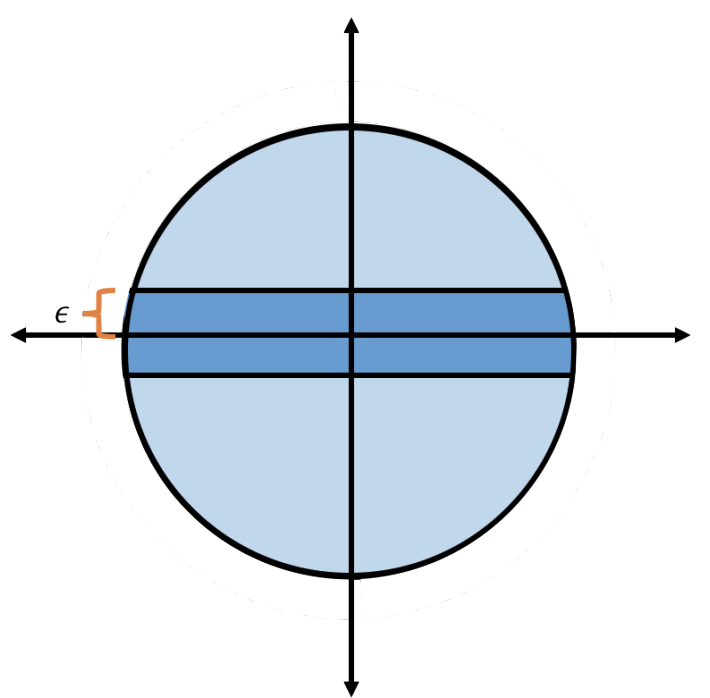
\includegraphics[width=.4\textwidth]{equator.png}
	\end{center}

	\begin{enumerate}
		\item Prove that with high probability, the first entry of $\bv{g}/\sqrt{d}$ is small. 
		\item Prove that $\bv{g}/\sqrt{d}$ is very very close to $\bv{g}/\|\bv{g}\|_2^2$, so this vector also has small first entry.
	\end{enumerate}
\end{frame}

\begin{frame}[t]
	\frametitle{concentration at equator}
	Let $\bv{g}$ be a random Gaussian vector and $\bv{w} = \bv{g}/\|\bv{g}\|_2$. 
	\begin{itemize}
		\item $\E[\|\bv{g}\|_2^2] = $
		\vspace{3em}
	\end{itemize} 
\textbf{Excersize for home:} Prove that $\Pr\left[\|\bv{g}\|_2^2\leq \frac{1}{2}\E[\|\bv{g}\|_2^2]\right] \leq 2^{-\Theta(d)}$. 

This should intuitively make sense. Can  you tell me why?
\end{frame}

\begin{frame}[t]
	\frametitle{concentration at equator}
	For $1 - 2^{-\Theta(d)}$ fraction of vectors $\bv{g}$, $\|\bv{g}\|_2 \geq \sqrt{d/2}$. Condition on the event that we get a random vector in this set. 
	
	Recall that $\bv{w} = \frac{\bv{g}}{\|\bv{g}\|_2}$. Given this event:
	\begin{align*}
	\Pr\left[|{w}_1| \leq \epsilon\right] &= \Pr\left[|g_1/\|\bv{g}\|_2| \leq \epsilon\right]\\
	&\geq \Pr\left[|g_1|/\sqrt{d/2} \leq \epsilon \right]\\
	&= \Pr\left[|g_1| \leq \epsilon\cdot \sqrt{d/2} \right]\\
	&\geq 1 - 2^{-\theta\left((\epsilon\cdot \sqrt{d/2})^2\right)}
	\end{align*}

	By union bound, overall we have:
	\begin{align*}
		\Pr\left[|{w}_1| \leq \epsilon\right] \geq 1 - 2^{-\Theta\left(\epsilon^2d\right)} - 2^{-\theta(d)}
	\end{align*}

\end{frame}

\begin{frame}[t]
	\frametitle{bizarre shape of unit ball}
	\begin{enumerate}
		\item $(1 -2^{-\Theta(\epsilon d)})$ fraction of volume lies $\epsilon$ close to surface. 
		\item $(1 - 2^{-\Theta(\epsilon^2 d)})$ fraction of volume lies $\epsilon$ close to any equator. 
	\end{enumerate}
	
	\begin{center}
		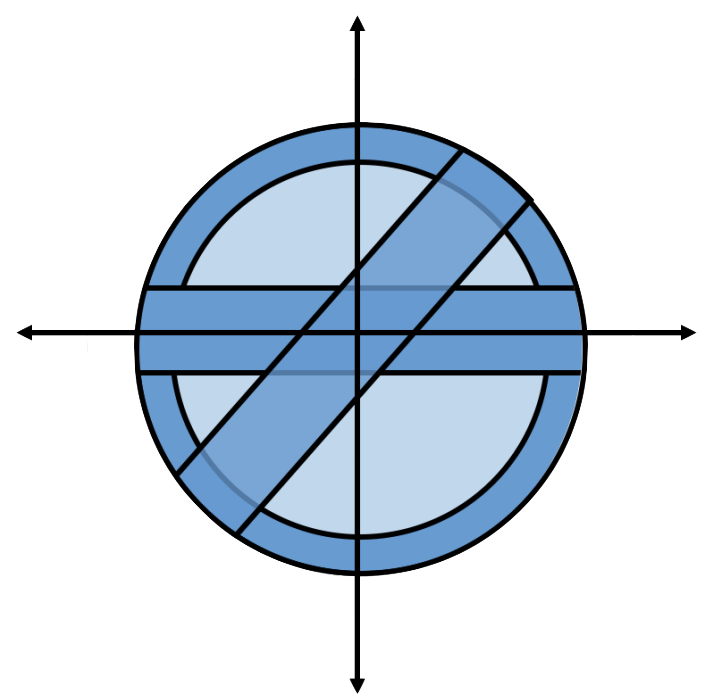
\includegraphics[width=.5\textwidth]{equators_surface.png}
		
		\alert{\textbf{High-dimensional ball looks nothing like 2D ball!}} 
	\end{center}
\end{frame}




\begin{frame}[t]
	\frametitle{high dimensional cube}
	Let $\mathcal{C}_d$ be the $d$-dimensional cube: 
	\begin{align*}
	\mathcal{C}_d = \{\bv{x}\in \R^d : |\bv{x}(i)| \leq 1 \,\, \forall i\}. 
	\end{align*}
	\begin{center}
		\vspace{-1em}
		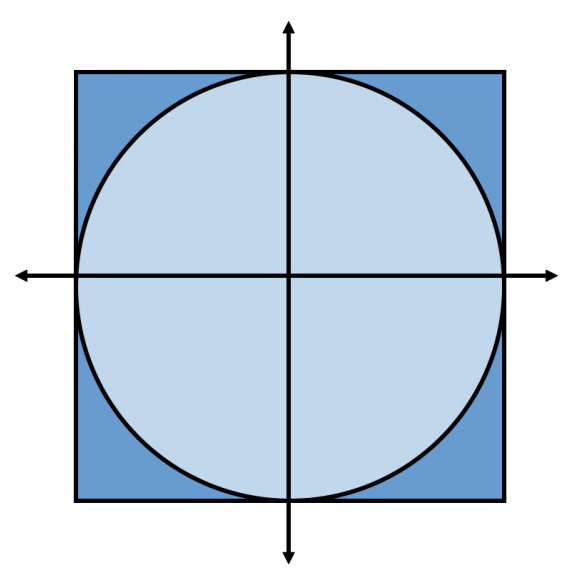
\includegraphics[width=.4\textwidth]{2dcube.png}
		
		\vspace{-.5em}
		In two dimensions, the cube is pretty similar to the ball. 
		
			But volume of $\mathcal{C}_d$ is $2^d$ while volume of unit ball is $\frac{\sqrt{\pi}^{d}}{(d/2)!}.$ 
			
			\alert{\textbf{This is a huge gap!}} Cube has $O(d)^{O(d)}$ more volume.
	\end{center}
\end{frame}

\begin{frame}
	\frametitle{high dimensional cube}
	Some other ways to see these shapes are very different:
	\begin{itemize}
		\item $\max_{\bv{x} \in \mathcal{B}_d} \|\bv{x}\|_2^2 = $
		\item $\max_{\bv{x} \in \mathcal{C}_d} \|\bv{x}\|_2^2 = $
	\end{itemize}
\end{frame}

\begin{frame}
	\frametitle{high dimensional cube}
	Some other ways to see these shapes are very different:
	\begin{itemize}
		\item $\E_{\bv{x} \sim \mathcal{B}_d} \|\bv{x}\|_2^2 $
		\item $\E_{\bv{x} \sim \mathcal{C}_d} \|\bv{x}\|_2^2 = $
	\end{itemize}
\end{frame}

\begin{frame}
	\frametitle{high dimensional cube}
	Almost all of the volume of the unit cube falls in its corners, and these corners lie far outside the unit ball. 
\begin{center}
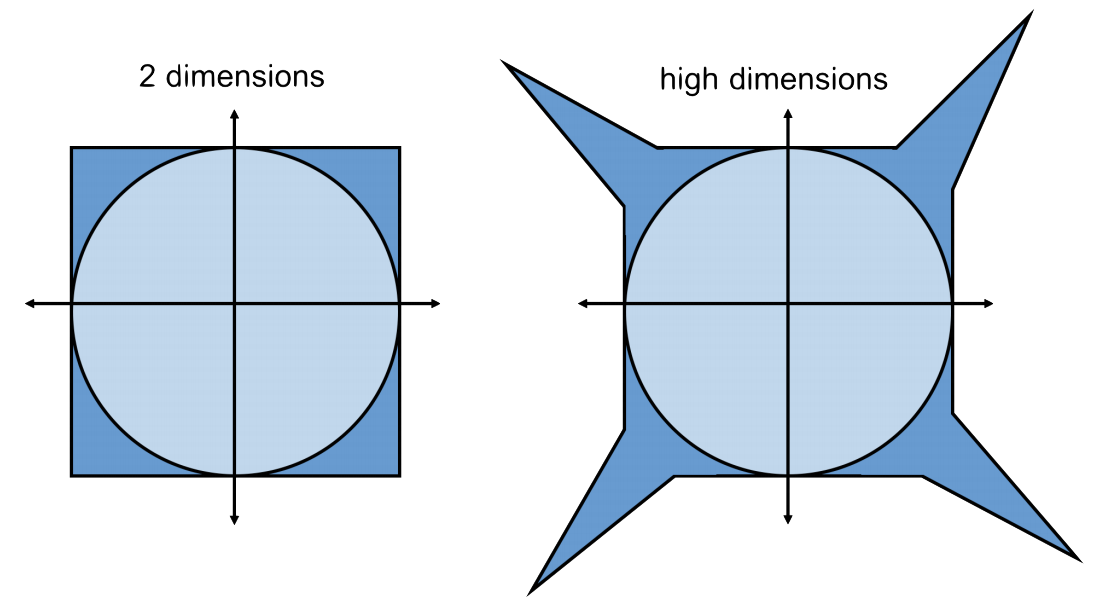
\includegraphics[width=.7\textwidth]{highdcube.png}
\end{center}
\end{frame}

\begin{frame}
	\frametitle{recent article}
	\begin{center}
	See \textbf{\textcolor{blue}{\href{https://www.quantamagazine.org/a-mathematicians-guided-tour-through-high-dimensions-20210913/}{The Journey to Define Dimension}}} from Quanta Magazine for another fun example comparing cubes to balls!
	\vspace{1em}
	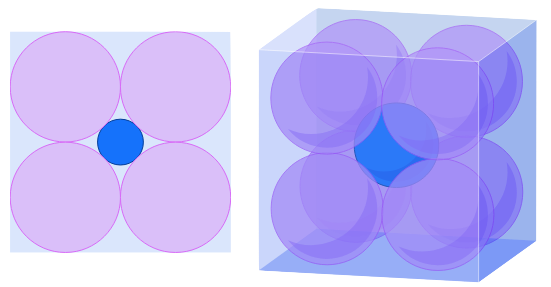
\includegraphics[width=.6\textwidth]{quanta.png}
	\end{center}
Place $2^d$ unit balls in box with side length $4$. Look at sphere they enclose. It has radius $\sqrt{d}-1$. 
\begin{center}
So for $d > 9$, it sticks out of the box...
\end{center}
\end{frame}

\begin{frame}
	\frametitle{dimensionality reduction}
	Despite \textbf{all this} warning that low-dimensional space looks nothing like high-dimensional space, next we are going to learn about how to \textbf{compress high dimensional vectors to low dimensions.} 
	
	We will be very careful not to compress things \emph{too} far. An extremely simple method known as Johnson-Lindenstrauss Random Projection pushes right up to the edge of how much compression is possible. 
\end{frame}


\begin{frame}
	\frametitle{euclidean dimensionality reduction}
	\begin{lemma}[Johnson-Lindenstrauss, 1984]
		For any set of $n$ data points $\bv{q}_1,\ldots, \bv{q}_n \in \R^d$ there exists a \emph{linear map} $\Pi: \R^d \rightarrow \R^k$ where $k = O\left(\frac{\log n}{\epsilon^2}\right)$ such that \emph{for all $i,j$},
		\begin{align*}
			(1-\epsilon)\|\bv{q}_i - \bv{q}_j\|_2 \leq \|\bs{\Pi}\bv{q}_i - \bs{\Pi}\bv{q}_j\|_2 \leq (1+\epsilon)\|\bv{q}_i - \bv{q}_j\|_2.
		\end{align*}
	\end{lemma}
	\begin{center}
		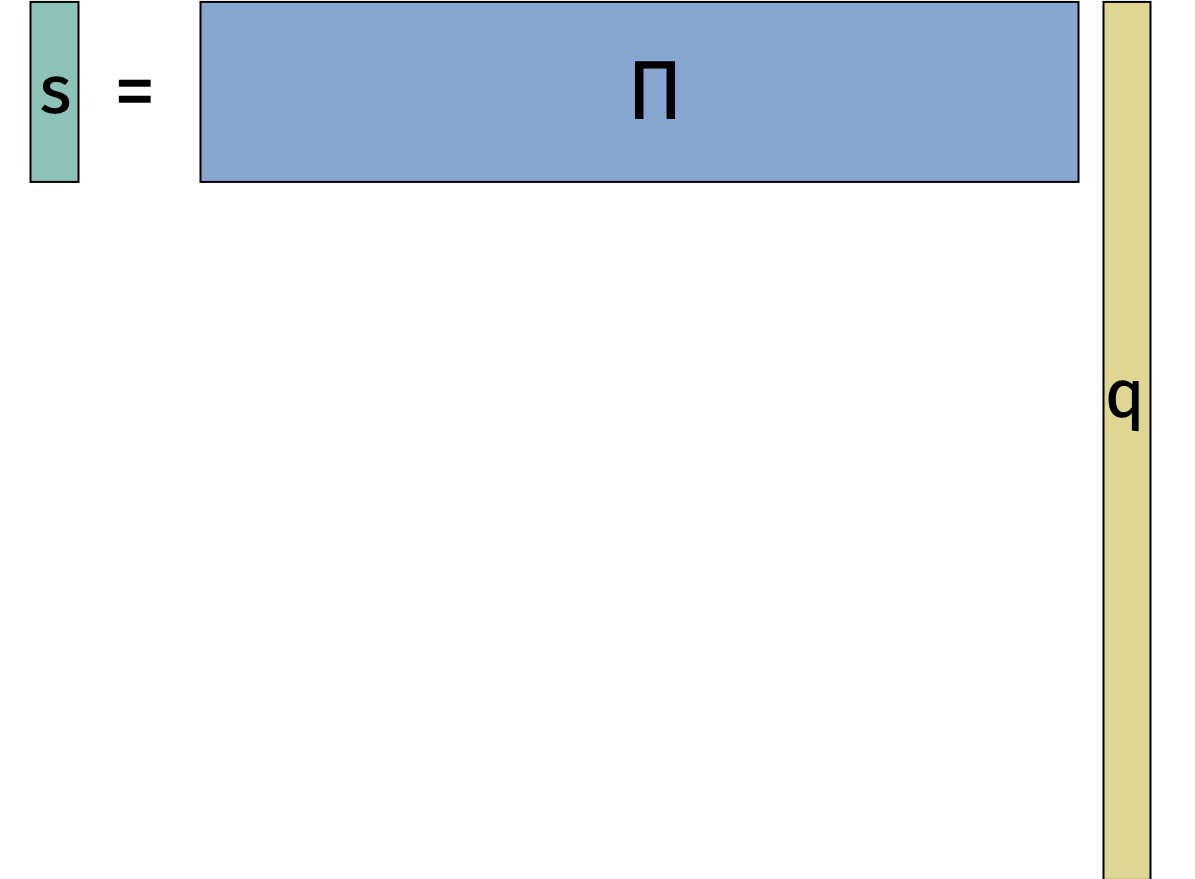
\includegraphics[height=.45\textheight]{jl_sketch.png}
	\end{center}
\end{frame}

\begin{frame}
	\frametitle{euclidean dimensionality reduction}
	This is equivalent to: 
	\begin{lemma}[Johnson-Lindenstrauss, 1984]
		For any set of $n$ data points $\bv{q}_1,\ldots, \bv{q}_n \in \R^d$ there exists a \emph{linear map} $\Pi: \R^d \rightarrow \R^k$ where $k = O\left(\frac{\log n}{\epsilon^2}\right)$ such that \emph{for all $i,j$},
		\begin{align*}
			(1-\epsilon)\|\bv{q}_i - \bv{q}_j\|_2^{\mathbf{\alert{2}}} \leq \|\bs{\Pi}\bv{q}_i - \bs{\Pi}\bv{q}_j\|_2^{\mathbf{\alert{2}}} \leq (1+\epsilon)\|\bv{q}_i - \bv{q}_j\|_2^{\mathbf{\alert{2}}}.
		\end{align*}
	\end{lemma}
	because for small $\epsilon$, $(1+\epsilon)^2 = 1 + O(\epsilon)$ and $(1-\epsilon)^2 = 1 - O(\epsilon)$.
\end{frame}

\begin{frame}
	\frametitle{tons of applications}
	\textbf{Make pretty much any computation involving vectors faster and more space efficient.}
	\begin{itemize}
		\item Faster vector search (used in image search, AI-based web search, Retrieval Augmented Generation (RAG), etc.).
		\item Faster machine learning (next class we will see an application to speeding up clustering).
		\item Faster numerical linear algebra. 
	\end{itemize}
	\begin{center}
		\alert{\textbf{Only useful if we can explicity construct a JL map $\bs{\Pi}$ and apply efficiently to vectors.}}
	\end{center}
\end{frame}

\begin{frame}
	\frametitle{euclidean dimensionality reduction}
	\begin{center}
		Remarkably, $\Pi$ can be chosen \emph{completely at random}!
	\end{center}
	\textbf{One possible construction:} Random Gaussian.
	\begin{align*}
		\bs{\Pi}_{i,j} = \frac{1}{\sqrt{k}} \mathcal{N}(0,1)
	\end{align*}
	The map $\bs{\Pi}$ is \textbf{\alert{oblivious to the data set}}. This stands in contrast to other vector compression methods you might know like PCA.
	
	[Indyk, Motwani 1998] [Arriage, Vempala 1999] [Achlioptas 2001] [Dasgupta, Gupta 2003].
	
	Many other possible choices suffice -- you can use random $\{+1,-1\}$ variables, sparse random matrices, pseudorandom $\Pi$. Each with different advantages. 
\end{frame}

\begin{frame}
	\frametitle{randomized jl constructions}
	\begin{center}
		Let $\bs{\Pi} \in \R^{k\times d}$ be chosen so that each entry equals $\frac{1}{\sqrt{k}}  \mathcal{N}(0,1)$.
		
		... or each entry equals $\frac{1}{\sqrt{k}}  \pm 1$ with equal probability.
	\end{center}
	\vspace{1em}
	
	\begin{columns}
		\begin{column}{0.5\textwidth}
			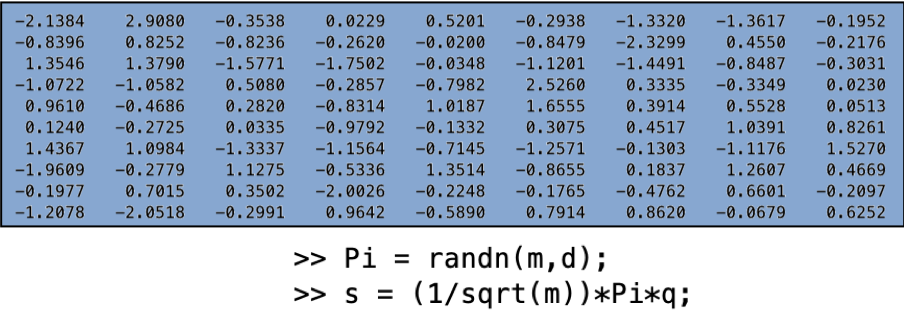
\includegraphics[width=\textwidth]{rand_gauss.png}
		\end{column}
		\begin{column}{0.5\textwidth}
			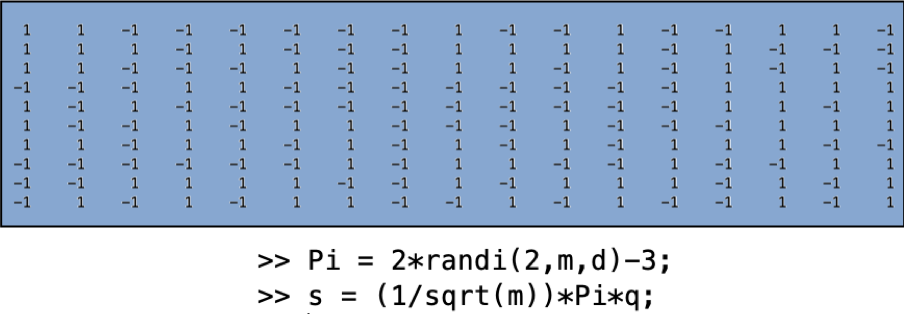
\includegraphics[width=\textwidth]{rand_sign.png}
		\end{column}
	\end{columns}
	
	\begin{center}
		A random orthogonal matrix $\bv{Q}$ also works. I.e. with $\bv{Q}\bv{Q}^T = \bv{I}_{k\times k}$. For this reason, the JL operation is often called a ``random projection", even though it technically is not a projection when $\bs{\Pi}'s$ entries are i.i.d.
	\end{center}
\end{frame}

\begin{frame}[t]
	\frametitle{random proection}
	Can anyone see why $\bs{\Pi}$ is similar to a projection matrix? I.e., a matrix satisfying  $\bv{Q}\bv{Q}^T = \bv{I}_{k\times k}$.
\end{frame}

\begin{frame}
	\frametitle{random projection}
	\begin{center}
		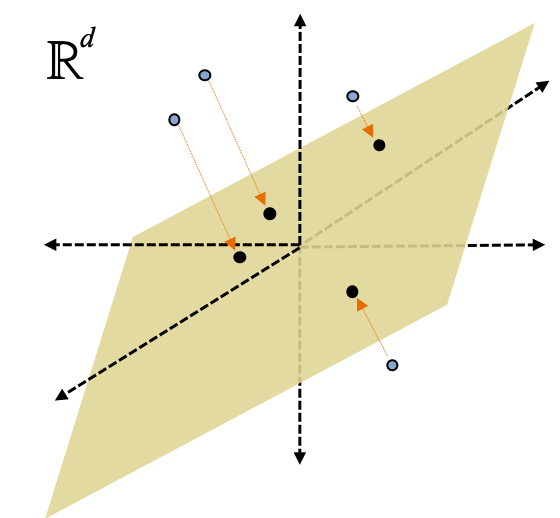
\includegraphics[width=.6\textwidth]{random_projection.png}
	\end{center}
	\textbf{Intuition:} Multiplying by a random matrix mimics the process of projecting onto a random $k$ dimensional subspace in $d$ dimensions.
\end{frame}

\begin{frame}
	\frametitle{euclidean dimensionality reduction}
	\textbf{Intermediate result:}
	\begin{lemma}[Distributional JL Lemma]
		Let $\bs{\Pi} \in \R^{k\times d}$ be chosen so that each entry equals $\frac{1}{\sqrt{k}}  \mathcal{N}(0,1)$, where $\mathcal{N}(0,1)$ denotes a standard Gaussian random variable. 
		
		If we choose $k = O\left(\frac{\log(1/\delta)}{\epsilon^2}\right)$, then for \emph{any vector $\bv{x}$}, with probability $(1-\delta)$:
		\begin{align*}
			(1-\epsilon)\|\bv{x}\|_2^2 \leq \|\bs{\Pi}\bv{x}\|_2^2 \leq (1+\epsilon) \|\bv{x}\|_2^2
		\end{align*}
	\end{lemma}
	
	\begin{center}\alert{
			\textbf{Given this lemma, how do we prove the traditional Johnson-Lindenstrauss lemma?}}
	\end{center}
\end{frame}

\begin{frame}
	\frametitle{jl from distributional jl}
	We have a set of vectors $\bv{q}_1, \ldots, \bv{q}_n$. Fix $i,j \in 1,\ldots, n$. 
	
	Let $\bv{x} = \bv{q}_i - \bv{q}_j$. By linearity, $\bs{\Pi}\bv{x} = \bs{\Pi}(\bv{q}_i - \bv{q}_j) = \bs{\Pi}\bv{q}_i - \bs{\Pi}\bv{q}_j$.
	
	By the Distributional JL Lemma, with probability $1-\delta$,
	\begin{align*}
		(1-\epsilon)\|\bv{q}_i - \bv{q}_j\|_2 \leq \|\bs{\Pi}\bv{q}_i - \bs{\Pi}\bv{q}_j\|_2 \leq (1+\epsilon) \|\bv{q}_i - \bv{q}_j\|_2.
	\end{align*}
	Finally, set $\delta = \frac{1}{n^2}$. Since there are $< n^2$ total $i,j$ pairs, by a union bound we have that with probability $9/10$, the above will hold \emph{for all} $i,j$, as long as we compress to:
	
	\begin{align*}
		k = O\left(\frac{\log(1/(1/n^2))}{\epsilon^2}\right) = O\left(\frac{\log n}{\epsilon^2}\right) \text{ dimensions.}\qed
	\end{align*}
	
\end{frame}

\begin{frame}
	\frametitle{proof of distributional jl}
	Want to argue that, with probability $(1-\delta)$,
	\begin{align*}
		(1-\epsilon)\|\bv{x}\|_2^2 \leq |\bs{\Pi}\bv{x}\|_2^2 \leq (1+\epsilon)\|\bv{x}\|_2^2 
	\end{align*}
	
	\begin{center}
		\alert{\textbf{Claim}: $\E \|\bs{\Pi} \bv{x} \|_2^2 = \|\bv{x}\|_2^2.$}
	\end{center}
	
	\vspace{-1em}
	Some notation:
	\begin{center}
		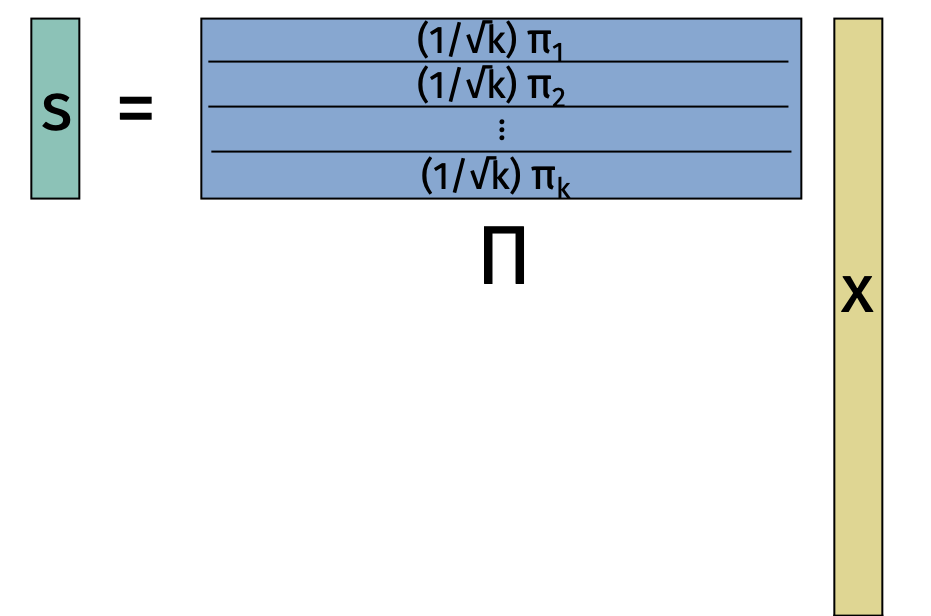
\includegraphics[width=.6\textwidth]{jl_notation.png}
		
		So each $\bs{\pi}_i$ contains $\mathcal{N}(0,1)$ entries. 
	\end{center}
\end{frame}

\begin{frame}
	\frametitle{proof of distributional jl}
	\textbf{Intermediate Claim:} Let $\bs{\pi}$ be a length $d$ vector with $\mathcal{N}(0,1)$ entries. 
	\begin{align*}
		\E\left[\|\bs{\Pi} \bv{x} \|_2^2 \right]  = \E\left[\left(\langle\bs{\pi},\bv{x}\rangle\right)^2 \right] .
	\end{align*}
	%	\begin{align*}
		%		\|\bs{\Pi} \bv{x} \|_2^2 = \sum_i^k \bv{s}[i]^2 = \sum_i^k \left(\frac{1}{\sqrt{k}}\langle\bs{\pi}_i,\bv{x}\rangle\right)^2 = \frac{1}{k}\sum_i^k \left(\langle\bs{\pi}_i,\bv{x}\rangle\right)^2 
		%	\end{align*}
	%	\begin{align*}
		%		\E\left[\|\bs{\Pi} \bv{x} \|_2^2 \right] &= \frac{1}{k}\sum_i^k \E\left[\left(\langle\bs{\pi}_i,\bv{x}\rangle\right)^2 \right] \\
		%		& =\E\left[\left(\langle\bs{\pi}_i,\bv{x}\rangle\right)^2 \right] 
		%	\end{align*}
	\vspace{9em}
	\begin{block}{\vspace*{-3ex}}
		\small \textbf{Goal}: Prove $\E \|\bs{\Pi} \bv{x} \|_2^2 = \|\bv{x}\|_2^2$.
	\end{block}
\end{frame}

\begin{frame}
	\frametitle{proof of distributional jl}	
	\begin{align*}
		\langle\bs{\pi},\bv{x}\rangle = Z_1\cdot{x}[1] + Z_2\cdot{x}[2]  +  \ldots + Z_d\cdot{x}[d]
	\end{align*}
	where each $Z_1, \ldots, Z_d$ is a standard normal $\mathcal{N}(0,1)$. 
	
	We have that $Z_i \cdot{x}[i]$ is a normal $\mathcal{N}(0,{x}[i]^2)$ random variable.
	
	\vspace{5em}
	\begin{block}{\vspace*{-3ex}}
		\small \textbf{Goal}: Prove $\E \|\bs{\Pi} \bv{x} \|_2^2 = \|\bv{x}\|_2^2$. Established: $\E \|\bs{\Pi} \bv{x} \|_2^2 = \E\left[\left(\langle\bs{\pi},\bv{x}\rangle\right)^2 \right]$
	\end{block}
\end{frame}

\begin{frame}[t]
	\frametitle{stable random variables}
	\textbf{What type of random variable is $\langle\bs{\pi},\bv{x}\rangle$?}
	\begin{fact}[Stability of Gaussian random variables]
		\begin{align*}
			\mathcal{N}(\mu_1, \sigma_1^2) + \mathcal{N}(\mu_2, \sigma_2^2) =  \mathcal{N}(\mu_1 + \mu_2, \sigma_1^2 + \sigma_2^2)
		\end{align*}
	\end{fact}
	\begin{align*}
		\langle\bs{\pi},\bv{x}\rangle &= \mathcal{N}(0,{x}[1]^2) + \mathcal{N}(0,{x}[2]^2) + \ldots + \mathcal{N}(0,{x}[d]^2) \\ &= \mathcal{N}(0,\|\bv{x}\|_2^2). 
	\end{align*}
	
	So $\E \|\bs{\Pi} \bv{x} \|_2^2 = \E\left[\left(\langle\bs{\pi},\bv{x}\rangle\right)^2 \right] = \E\left[\mathcal{N}(0,\|\bv{x}\|_2^2)\right]  = \|\bv{x}\|_2^2$, as desired.
\end{frame}

\begin{frame}
	\frametitle{proof of distributional jl}
	Want to argue that, with probability $(1-\delta)$,
	\begin{align*}
		(1-\epsilon)\|\bv{x}\|_2^2 \leq \|\bs{\Pi}\bv{x}\|_2^2 \leq (1+\epsilon)\|\bv{x}\|_2^2 
	\end{align*}
	
	\begin{enumerate}
		\item $\E \|\bs{\Pi} \bv{x} \|_2^2 = \|\bv{x}\|_2^2$.
		\item Need to use a concentration bound.
	\end{enumerate}
	\begin{align*}
		\|\bs{\Pi} \bv{x} \|_2^2 = \frac{1}{k}\sum_{i=1}^k \left(\langle\bs{\pi}_i,\bv{x}\rangle\right)^2 = \frac{1}{k}\sum_{i=1}^k \mathcal{N}(0,\|\bv{x}\|_2^2)
	\end{align*}
	\alert{``Chi-squared random variable with $k$ degrees of freedom.''}
\end{frame}

\begin{frame}[t]
	\frametitle{concentration of chi-squared random variables}
	\begin{lemma} Let $H$ be a Chi-squared random variable with $k$ degrees of freedom. 
		\begin{align*}
			\Pr[|\E H - H| \geq \epsilon \E H] \leq 2 e^{-k\epsilon^2/8}
		\end{align*}
	\end{lemma}
	
	\vspace{8em}
	\begin{block}{\vspace*{-3ex}}
		\small \textbf{Goal}: Prove $\|\bs{\Pi} \bv{x} \|_2^2$ concentrates within $1 \pm \epsilon$ of its expectation, which equals $\|\bv{x} \|_2^2$.
	\end{block}
\end{frame}

\begin{frame}
	\frametitle{connection to earlier part of lecture}
	If high dimensional geometry is so different from low-dimensional geometry, why is \emph{dimensionality reduction possible?} 
	
	Doesn't Johnson-Lindenstrauss tell us that high-dimensional geometry can be approximated in low dimensions?
\end{frame}

\begin{frame}[t]
	\frametitle{connection to dimensionality reduction}
	\textbf{Hard case:} $\bv{x}_1, \ldots, \bv{x}_n \in \R^d$ are all mutually orthogonal unit vectors: 
	\begin{align*}
		\|\bv{x}_i - \bv{x}_j\|_2^2 &= 2 & &\text{for all $i,j$.}  
	\end{align*}
	When we reduce to $k$ dimensions with JL, we still expect these vectors to be nearly orthogonal. Why?
	
\end{frame}

\begin{frame}[t]
	\frametitle{connection to dimensionality reduction}
	\textbf{Hard case:} $\bv{x}_1, \ldots, \bv{x}_n \in \R^d$ are all mutually orthogonal unit vectors: 
	\begin{align*}
		\|\bv{x}_i - \bv{x}_j\|_2^2 &= 2 & &\text{for all $i,j$.}  
	\end{align*}
	
	From our result earlier, in $O(\log n /\epsilon^2)$ dimensions, there exists $2^{O(\epsilon^2\cdot \log n /\epsilon^2)} \geq n $ unit vectors that are close to mutually orthogonal.
	\alert{$O(\log n /\epsilon^2)$ = \emph{just enough} dimensions.}
	\vspace{2em}
	
	\textbf{Alternative view:} Without additional structure, we expect that learning/inference in $d$ dimensions requires $2^{O(d)}$ data points. If we really had a data set that large, then the JL bound would be vacous, since $\log(n) = O(d)$.
\end{frame}



\end{document} 




